	\documentclass{article}
			
		\usepackage{parskip}
		\usepackage{listings}
		\usepackage{xcolor}
		\usepackage{textcomp}
			
		%STYLE AND COLOR DEFINITION FOR SOURCE CODE 	
		\newcommand{\PHPamountofcolor}{75}
		\newcommand{\SourceCodeContext}{5}
		%Lets define the php language colors:
		\definecolor{PHP_comment_old}{HTML}{FF8000}
		\colorlet{PHP_comment}{PHP_comment_old!\PHPamountofcolor!black}
		\definecolor{PHP_default_old}{HTML}{000000}
		\colorlet{PHP_default}{PHP_default_old!\PHPamountofcolor!black}
		\definecolor{PHP_keyword_old}{HTML}{6c9c11}
		\colorlet{PHP_keyword}{PHP_keyword_old!\PHPamountofcolor!black}
		\definecolor{PHP_emph1_old}{HTML}{0F58A2}
		\colorlet{PHP_emph1}{PHP_emph1_old!\PHPamountofcolor!black}
		\definecolor{PHP_emph2_old}{HTML}{CCAA00}
		\colorlet{PHP_emph2}{PHP_emph2_old!\PHPamountofcolor!black}
		\definecolor{PHP_emph4_old}{HTML}{C60484}
		\colorlet{PHP_emph4}{PHP_emph4_old!\PHPamountofcolor!black}
		\definecolor{PHP_string_old}{HTML}{C78F0A}
		\colorlet{PHP_string}{PHP_string_old!\PHPamountofcolor!black}
		\definecolor{PHP_variable_old}{HTML}{C82210}%C82210
		\colorlet{PHP_variable}{PHP_variable_old!\PHPamountofcolor!black}
		\definecolor{PHP_number_old}{HTML}{BF1CA6}
		\colorlet{PHP_number}{PHP_number_old!\PHPamountofcolor!black}
		%Now we want to highlight the variables. This will be done by triggering the function \PHPhighlightvar at the start of any $ run. This function wil only highlight variables and any other identifiers will be ignored. Luckily lstlisting will only give correct identifiers so we only will have to check if the previous call was made with a $
		\usepackage{fontspec}
		\setmonofont{Courier}
		%\usepackage[utf8]{inputenc}
		%\usepackage[T1]{fontenc}
		%\usepackage{courier, textcomp}
		\usepackage{etoolbox}
		\newtoggle{InString}{}% Keep track of if we are within a string
		\togglefalse{InString}% Assume not initally in string
		
		\newcommand*{\ColorIfNotInString}[1]{\iftoggle{InString}{#1}{\color{PHP_number}#1}}%

		%helper
		
		\newcommand{\PHPhighlightvar}[1]{\ifnum\theDollarFlag=1 \color{PHP_variable} \fi#1\setcounter{DollarFlag}{0}}
		\newcounter{DollarFlag}
		
		%images
		\usepackage{graphicx}
		\graphicspath{ {images/} }
		\usepackage{wrapfig}
		\usepackage{subcaption}
		
		
			
			
			
		
			
			\title{Machine Learning: Fifth Home Work \\ \bigskip \large  Clustering with K-means and Gaussian Mixture Models}

			\author{Edoardo Ghini}
			
			\begin{document}
			
			\textbf{\maketitle}
			\pagenumbering{gobble}
			
			\bigskip\bigskip\bigskip
			\begin{center}
			
\includegraphics[width=0.5\textwidth]{laSapienza}
			\end{center}
			\bigskip\bigskip\bigskip
			\textbf{
			Dipartimento di Ingegneria dell'Università di Roma La Sapienza}
			

			\newpage
			\pagenumbering{roman}
			\tableofcontents
			\newpage
			\pagenumbering{arabic}
			
			
			
			
			
			%SETTING STYLE OF SOURCE CODE
			\lstset{
		  language        = php,
		  basicstyle      = \footnotesize\ttfamily,
		  keywordstyle    = \color{PHP_keyword},
		  stringstyle     = \color{PHP_string!90!black}\toggletrue{InString},
		  %this allows highlighting of variables:
		  literate        =  {\$}{{\iftoggle{InString}{\$}{\setcounter{DollarFlag}{1}\color{PHP_variable}\$\color{PHP_default}}}}1
		%    {"}{{{\ProcessQuote{"}}}}1% Disable coloring within double quotes
		%    {'}{{{\ProcessQuote{'}}}}1% Disable coloring within single quote
		    {0}{{{\ColorIfNotInString{0}}}}1
		    {1}{{{\ColorIfNotInString{1}}}}1
		    {2}{{{\ColorIfNotInString{2}}}}1
		    {3}{{{\ColorIfNotInString{3}}}}1
		    {4}{{{\ColorIfNotInString{4}}}}1
		    {5}{{{\ColorIfNotInString{5}}}}1
		    {6}{{{\ColorIfNotInString{6}}}}1
		    {7}{{{\ColorIfNotInString{7}}}}1
		    {8}{{{\ColorIfNotInString{8}}}}1
		    {9}{{{\ColorIfNotInString{9}}}}1,
		  identifierstyle = \color{PHP_default}\PHPhighlightvar,
		  commentstyle    = \color{PHP_comment}\slshape,
		  emph            =[1]{require_once, require, include_once, include, namespace, use, class, function, new},
		  emphstyle       =[1]\color{PHP_emph1},%\bf,
		  emph            =[2]{echo, empty, isset, array, instanceof},
		  emphstyle       =[2]\color{PHP_emph2},%\bf,
		  emph            =[3]{var, const, abstract, 
		                        protected, private, public,
		                        static, final, extends, implements,
		                        global, if, else, foreach ,for,
		                        endforeach, endif, endfor, elseif,
		                        as},
		  emphstyle       =[3]\color{PHP_keyword},%\bf,
		  emph            =[4]{return, throw, exit, __halt_compiler, continue, break},
		  emphstyle       =[4]\color{PHP_emph4},%\bf,
		  breaklines      = true,
		  captionpos      = b,
		  rulecolor       =\color{black},
		  keywords    ={__halt_compiler,    abstract,   and,    array,
		                    as, break,  callable,   case,   catch,  class,
		                    clone,  const,  continue,   declare,    default,
		                    die,    do, echo,   else,   elseif,
		                    empty,  enddeclare, endfor, endforeach, endif,
		                    endswitch,  endwhile,   eval,   exit,   extends,
		                    final,  finally,    for,    foreach,    function,
		                    global, goto, if,   implements, include,
		                    include_once,   instanceof, insteadof,
		                    interface,  isset, list,    namespace,
		                    new,    or, print, private, protected,  public,
		                    require,    require_once, return,   static,
		                    switch, throw,  trait, try, unset, use, var,
		                    while,  xor,    yield,
		  },
		  numbers=left,
		  stepnumber=1,  
		  numberfirstline=true,
		  numberstyle=\footnotesize,
		  xleftmargin=4.0ex,
		  upquote=true,
		  showlines=true
		  }	
			
			\renewcommand{\lstlistingname}{Code}

			
			\part{Introduction}
			
				\section{Scope}
Familiarise with unsupervised techniques to analyse datas.
				\section{Objectives}
				The assignment consider the usage of two effective approaches to clustering problems and an analysis of the results with three different metrics.
				\begin{center}
\begin{figure}
\centering
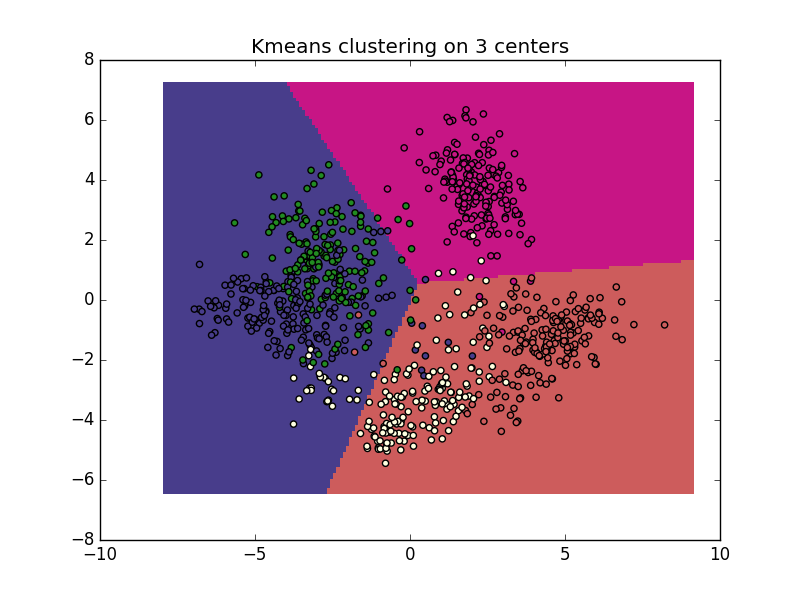
\includegraphics[width=0.9\textwidth]{figure_1}
\caption{}
\label{fig:1}
\end{figure}
\end{center}

\newpage
			\part{Development}
				\section{Data Manipulations}
	
	At the beginning I had to load a dataset and applying a principal component analysis extracting the first two most significative vectors of data in order to being able to visualise them on a two-dimensional space.
	

				\section{Clusterization}
				\subsection{Kmeans}
				\subsubsection{Execution}
				At first, I iterated the Kmeans algorithm changing the number of clusters to define, as can be seen from the plots.
		
								\begin{center}
				\begin{figure}
\centering
        \begin{subfigure}[b]{0.48\textwidth}
                \centering
                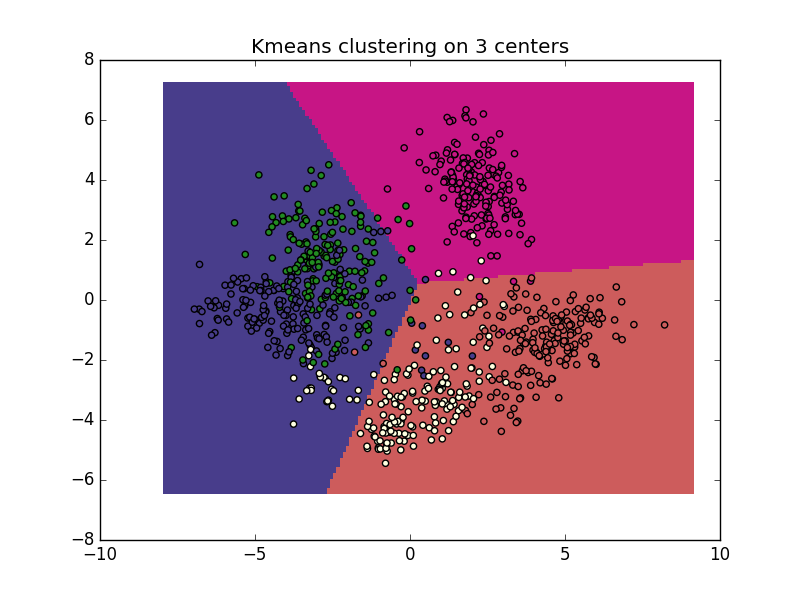
\includegraphics[width=\linewidth]{figure_1}
        \end{subfigure}\hfill
        \begin{subfigure}[b]{0.48\textwidth}
                \centering
                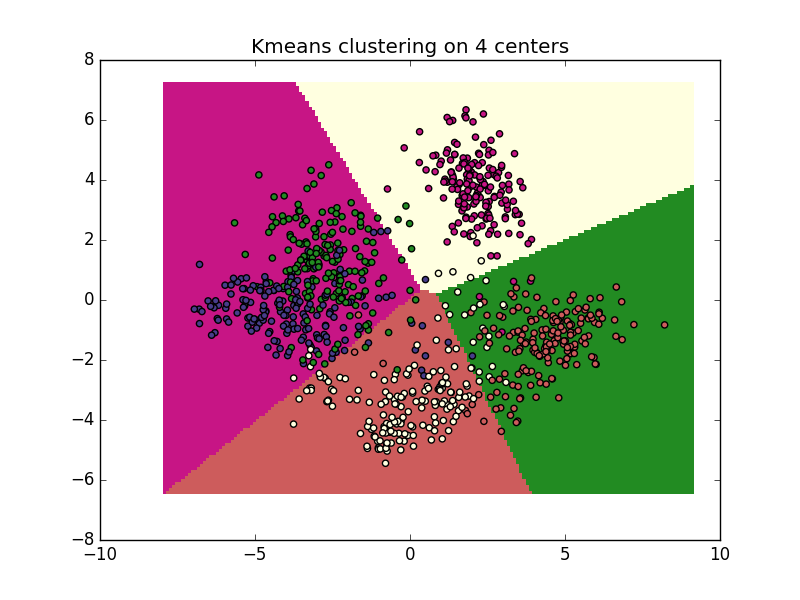
\includegraphics[width=\linewidth]{figure_2}
        \end{subfigure}\hfill
 \label{fig:1}
 \end{figure}
       
\begin{figure}
\centering  
        \begin{subfigure}[b]{0.48\textwidth}
                \centering
                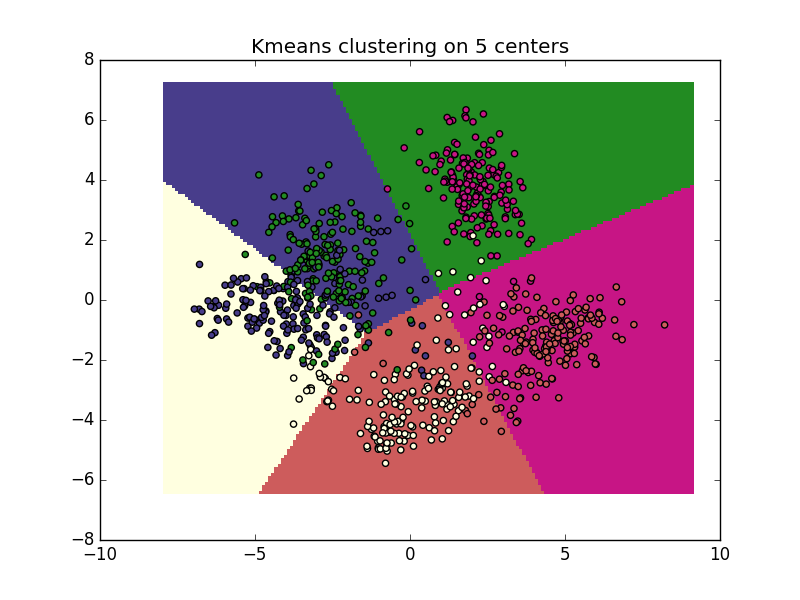
\includegraphics[width=\linewidth]{figure_3}
        \end{subfigure}\hfill
        \begin{subfigure}[b]{0.48\textwidth}
                \centering
                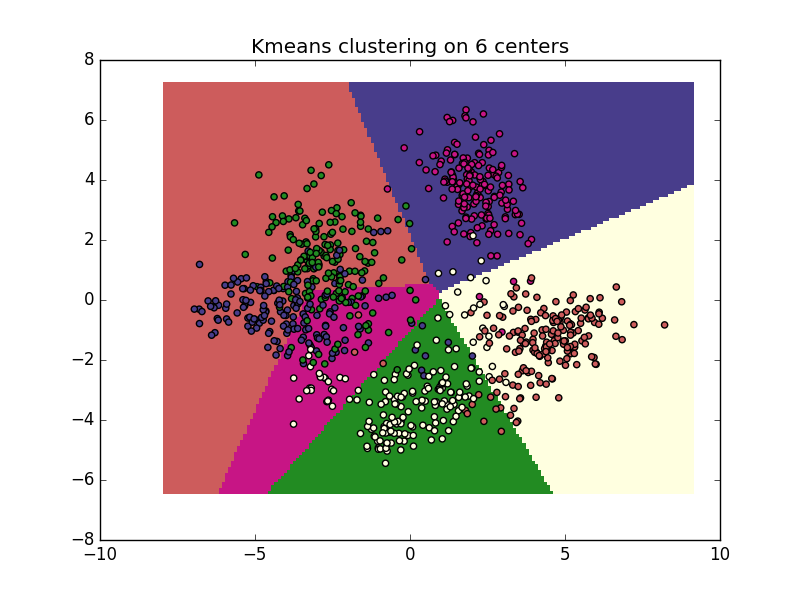
\includegraphics[width=\linewidth]{figure_4}
        \end{subfigure}
        \label{fig:2}
\end{figure}

\begin{figure}
\centering
        \begin{subfigure}[b]{0.48\textwidth}
                \centering
                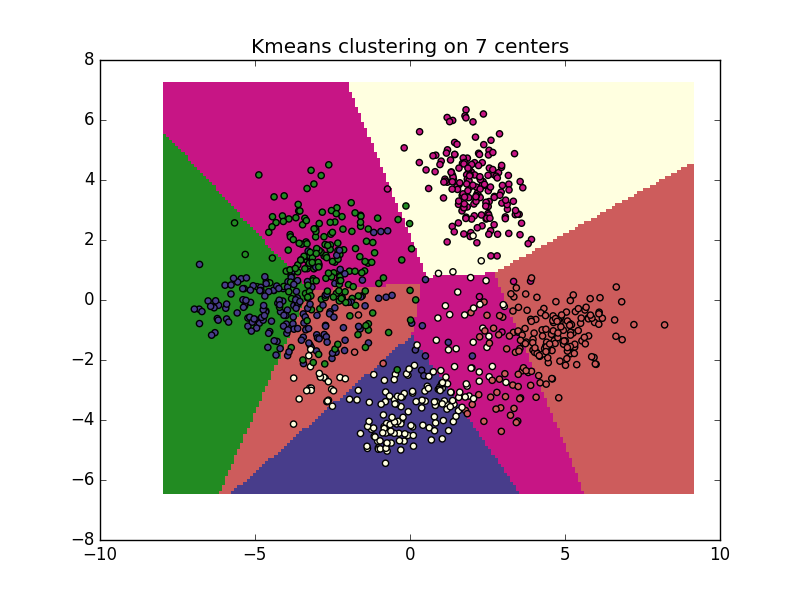
\includegraphics[width=\linewidth]{figure_5}
        \end{subfigure}\hfill
        \begin{subfigure}[b]{0.48\textwidth}
                \centering
                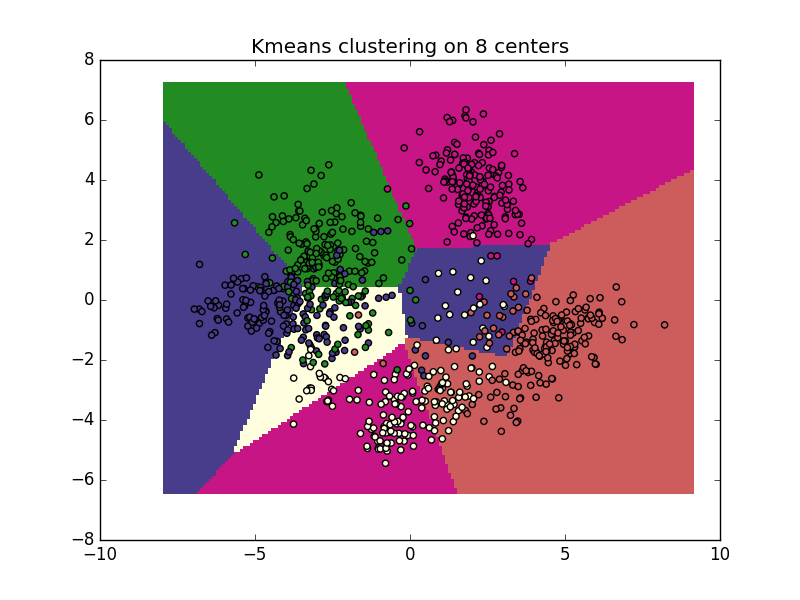
\includegraphics[width=\linewidth]{figure_6}
        \end{subfigure}\hfill
        \label{fig:3}
 \end{figure}
       
\begin{figure}
\centering  
        \begin{subfigure}[b]{0.48\textwidth}
                \centering
                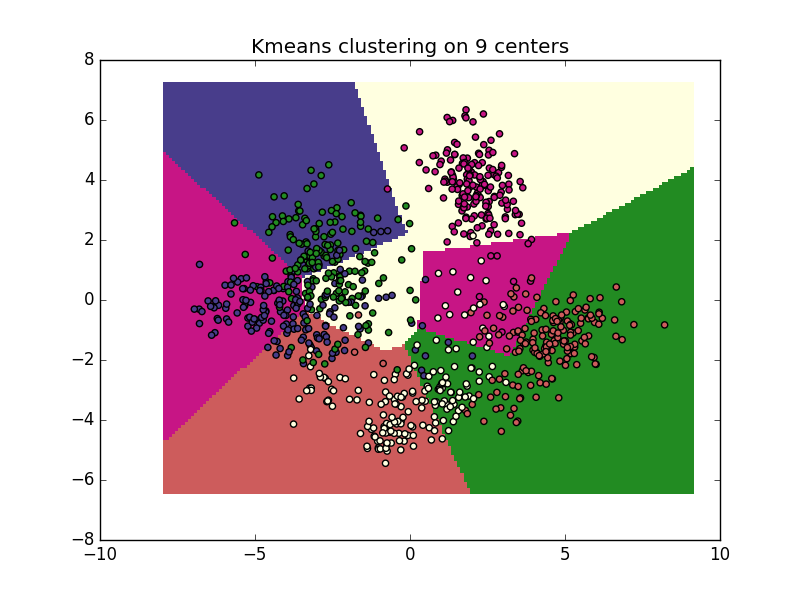
\includegraphics[width=\linewidth]{figure_7}
        \end{subfigure}\hfill
        \begin{subfigure}[b]{0.48\textwidth}
                \centering
                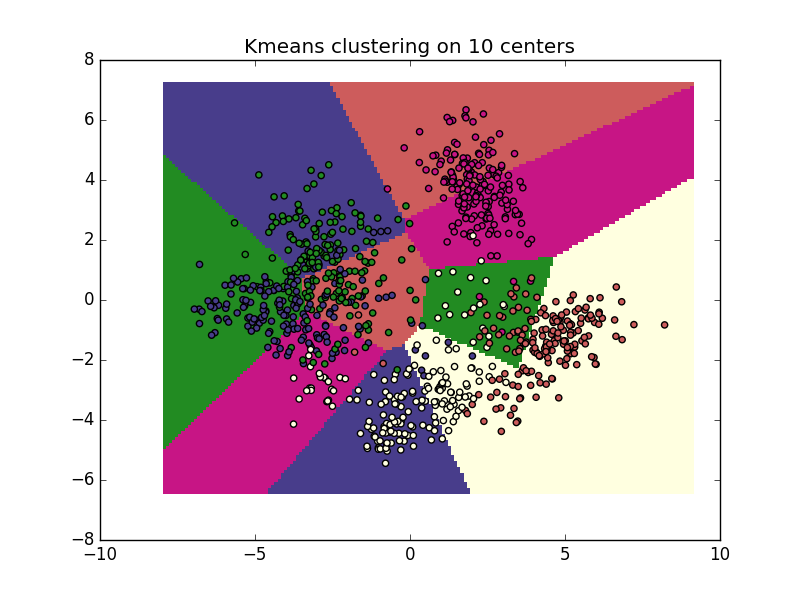
\includegraphics[width=\linewidth]{figure_8}
        \end{subfigure}
        \label{fig:4}
\end{figure}
\end{center}			 
			
				
				
				


				\subsubsection{Score Analysis}
				After the iteration was completed, I applied three different metrics to evaluate the effectiveness of the model feeding the evaluators with the predictions coming from the model and the true labels of the data.
				In fig(5) there are the results.
				
				\subsection{GMM}
				\subsubsection{Execution}
				In this other case, I made the same iteration as before, but this time I adopted an approach based on a Gaussian Mixture Model. This strategy allows to define non-linear boundaries of the clusters, therefore it brings more flexibility finding the best separators between clusters. The following plots show how the GMM recognise different numbers of clusters within data.
											\begin{center}
				\begin{figure}
\centering
        \begin{subfigure}[b]{0.48\textwidth}
                \centering
                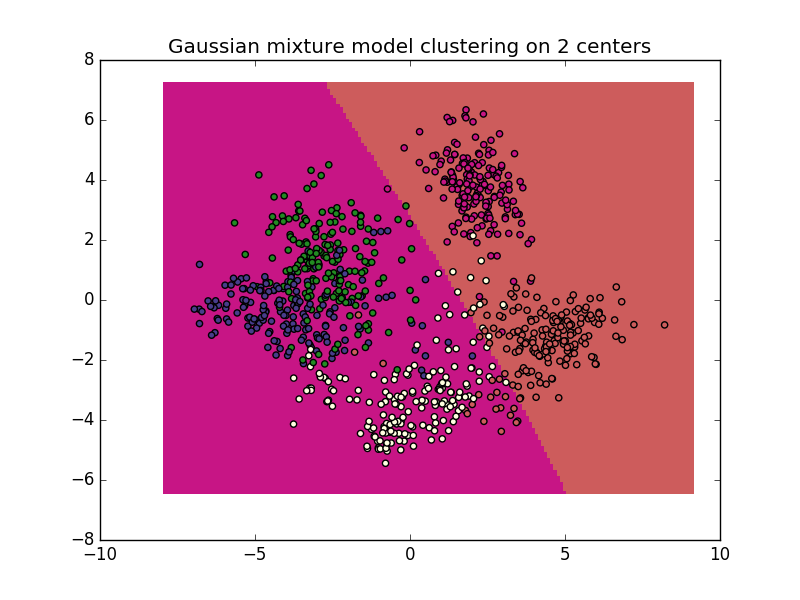
\includegraphics[width=\linewidth]{figure_10}
        \end{subfigure}\hfill
        \begin{subfigure}[b]{0.48\textwidth}
                \centering
                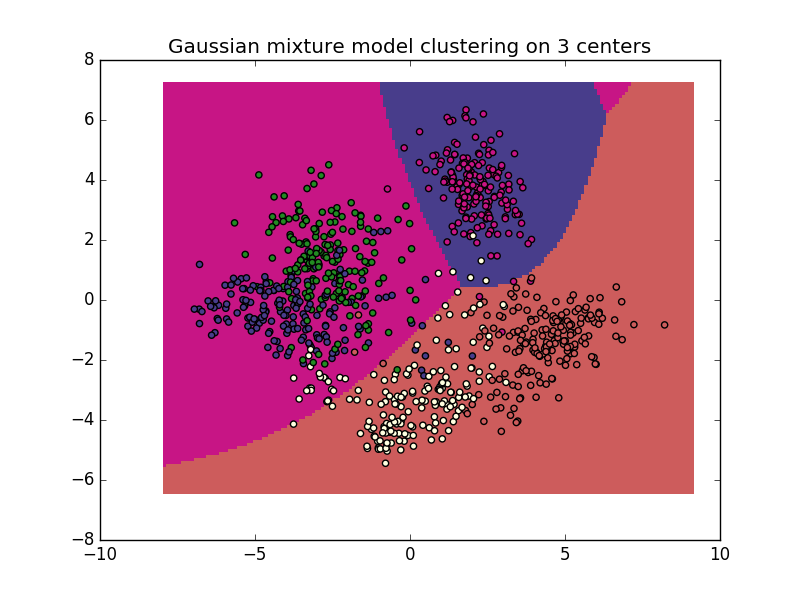
\includegraphics[width=\linewidth]{figure_11}
        \end{subfigure}\hfill
 \label{fig:5}
 \end{figure}
       
\begin{figure}
\centering  
        \begin{subfigure}[b]{0.48\textwidth}
                \centering
                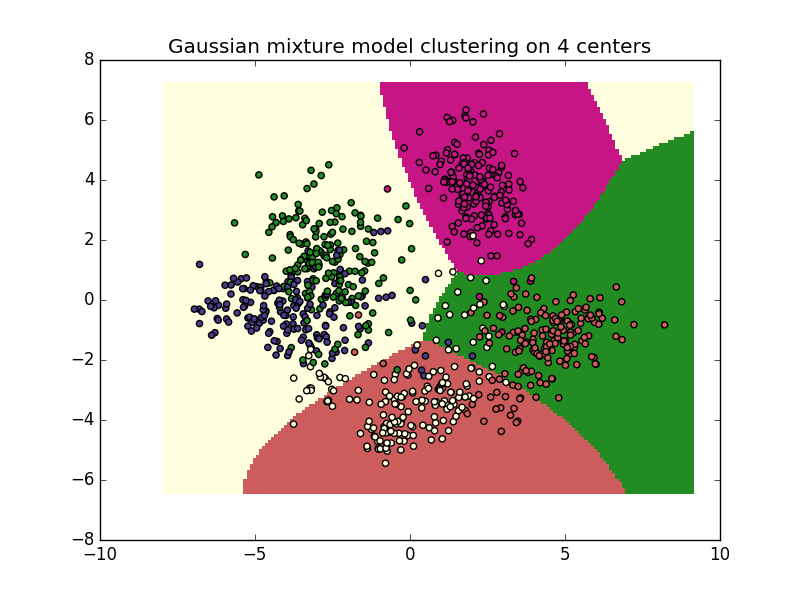
\includegraphics[width=\linewidth]{figure_12}
        \end{subfigure}\hfill
        \begin{subfigure}[b]{0.48\textwidth}
                \centering
                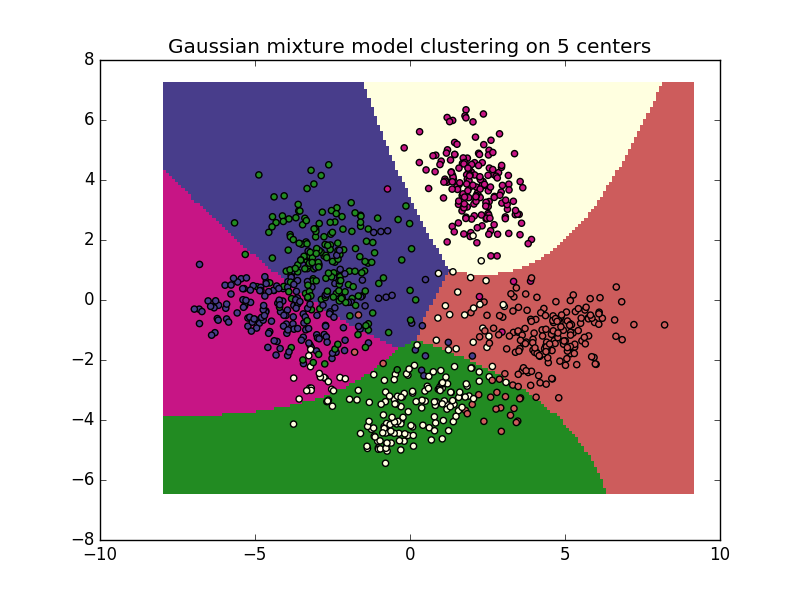
\includegraphics[width=\linewidth]{figure_13}
        \end{subfigure}
        \label{fig:6}
\end{figure}

\begin{figure}
\centering
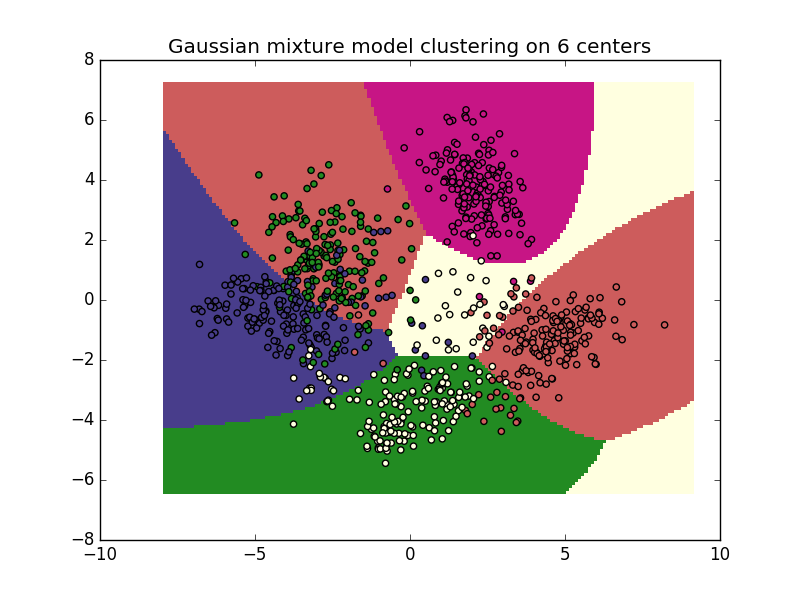
\includegraphics[width=0.9\textwidth]{figure_14}
\caption{}
\label{fig:7}
\end{figure}


\begin{figure}
\centering
        \begin{subfigure}[b]{0.48\textwidth}
                \centering
                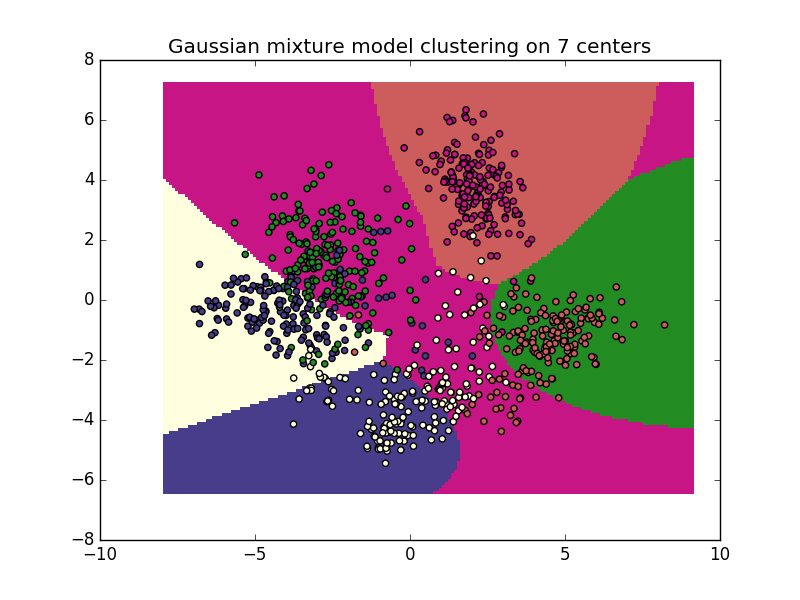
\includegraphics[width=\linewidth]{figure_15}
        \end{subfigure}\hfill
        \begin{subfigure}[b]{0.48\textwidth}
                \centering
                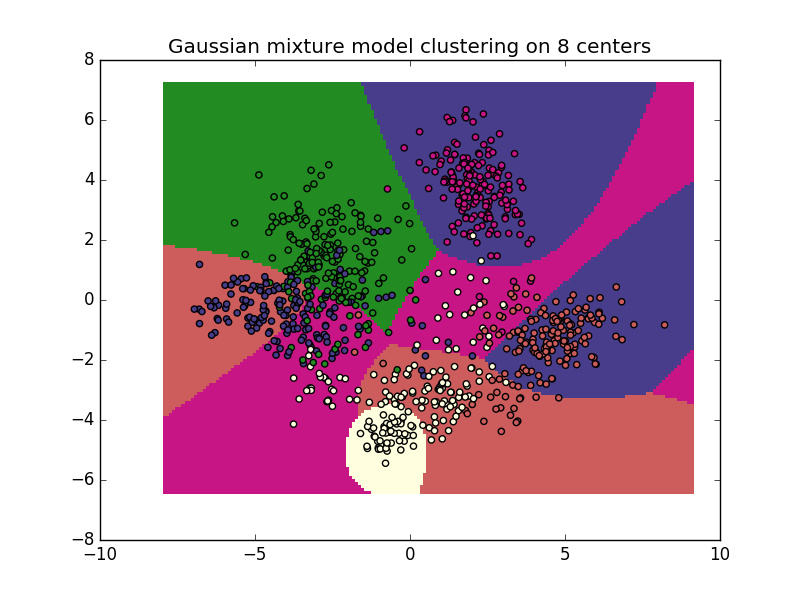
\includegraphics[width=\linewidth]{figure_16}
        \end{subfigure}\hfill
        \label{fig:8}
 \end{figure}
       
\begin{figure}
\centering  
        \begin{subfigure}[b]{0.48\textwidth}
                \centering
                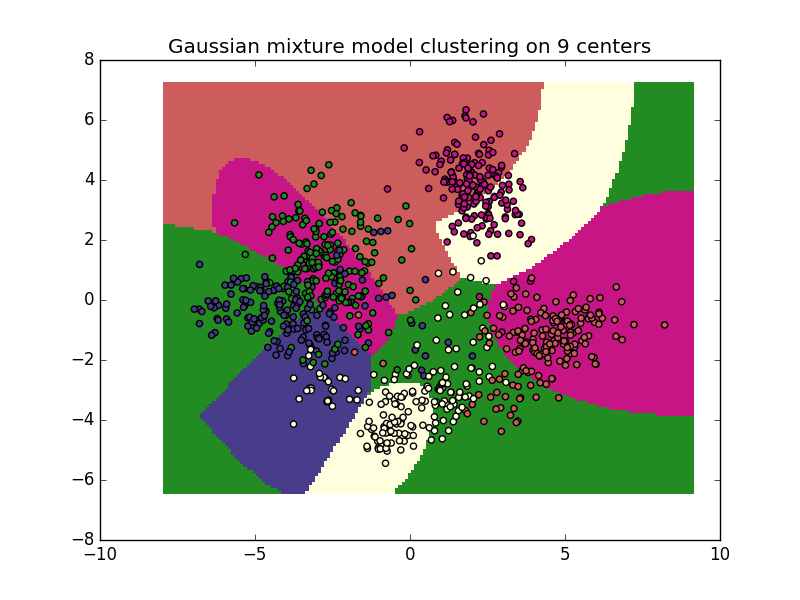
\includegraphics[width=\linewidth]{figure_17}
        \end{subfigure}\hfill
        \begin{subfigure}[b]{0.48\textwidth}
                \centering
                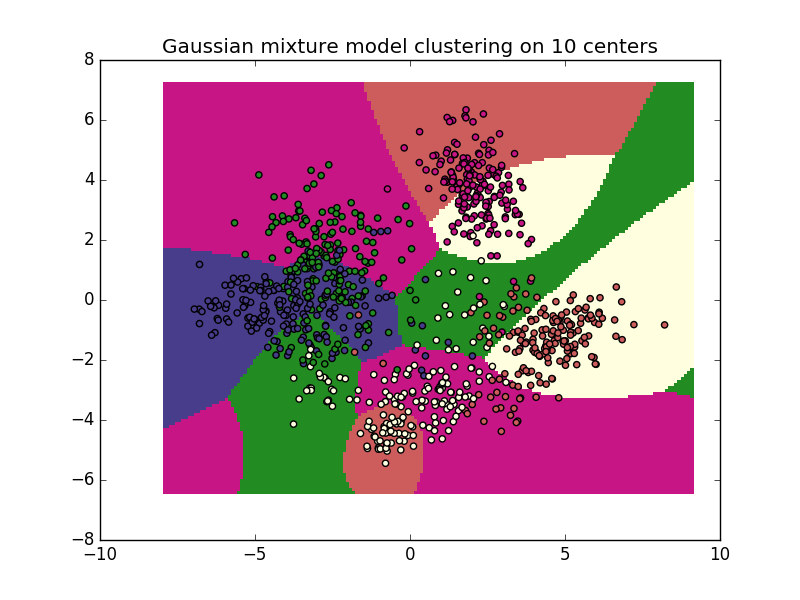
\includegraphics[width=\linewidth]{figure_18}
        \end{subfigure}
        \label{fig:9}
\end{figure}
\end{center}	
				\subsubsection{Score Analysis}
				In the same fashion as before, in fig(10) there are results about three different metric evaluations according to predicted and real labels.
\begin{center}
\begin{figure}
\centering
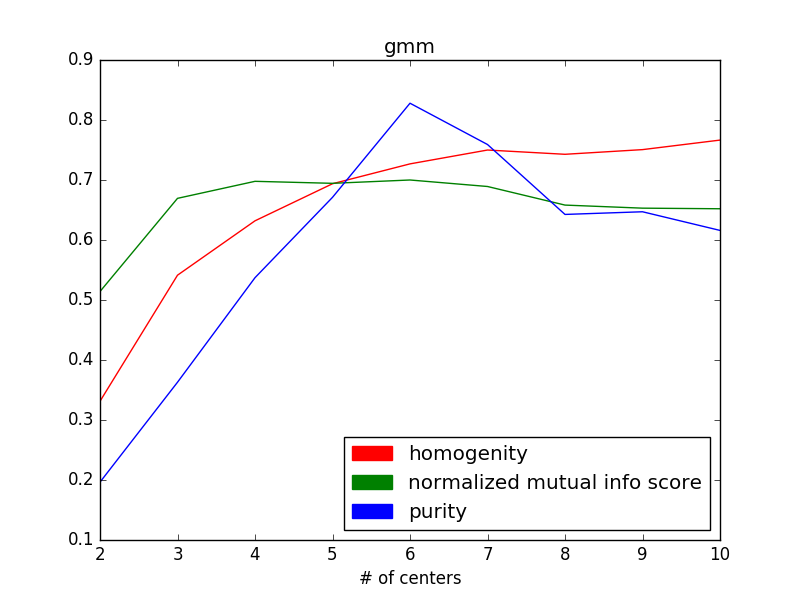
\includegraphics[width=0.9\textwidth]{figure_19}
\caption{}
\label{fig:10}
\end{figure}
\end{center}
				
\newpage
			\part{Conclusions}
			In the final analysis the best score of the various experiments is extremely metric-dependent.
			In fact, the metric choice is a major concern when we are dealing with unsupervised learning.
			For this particular case,  the purity seems to be the highest considering only six clusters.\\\smallskip
			 Finally, the three metric scores have similar behaviour with the variation of the number of cluster in the respect of both the approaches ( Kmeans and GMM).
		\end{document}
